\subsection{Collectivity and Flow (Wei)}

An important point that should be kept in mind is that the very events
showing strong collectivity in small systems are in a class of their own.
They represent a small fraction of the total cross-section with highest particle
multiplicities. 

The rareness of these high-multiplicity events pose quests of future high-luminosity pPb runs.
Based on the approximate KNO scaling of multiplicity distributions at various collision energies,
a projected multiplicity distribution for pPb collisions at \rootsNN\ = 8.16 TeV is shown
in Fig.~\ref{fig:Ntrk_pPb}, with an integrated luminosity of 100 nb$^{-1}$


Events with 100--200 tracks (these are the high-multiplicity events
where a ridge signal is seen in pp and pPb) are a common occurrence in
PbPb. 


\begin{figure}[thb]
  \begin{center}
    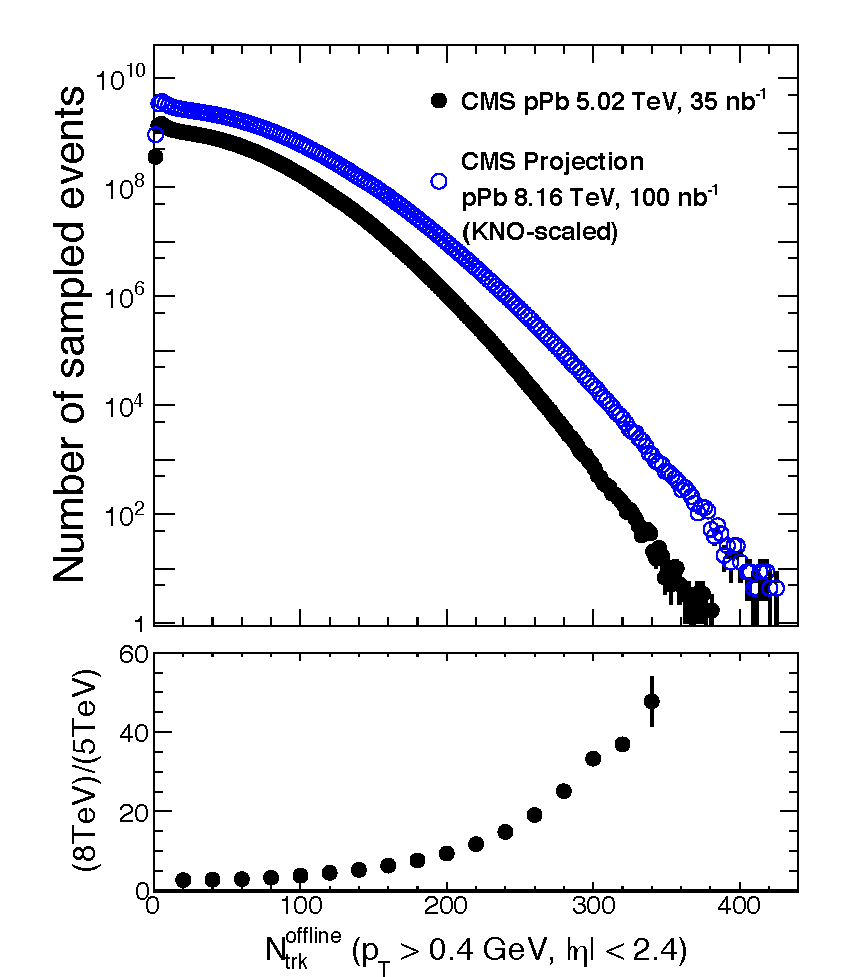
\includegraphics[width=0.5\textwidth]{figures/Ntrk.pdf}
    \caption{ Projected charged particle multiplicity distribution for pPb collisions at \rootsNN\ = 8.16 TeV
    with L$_{\rm int}$ = 100 nb$^{-1}$
    based on KNO scaling of measured distribution at \rootsNN\ = 5.02 TeV.
    }
    \label{fig:Ntrk_pPb}
  \end{center}
\end{figure} 

\begin{figure}[thb]
  \begin{center}
    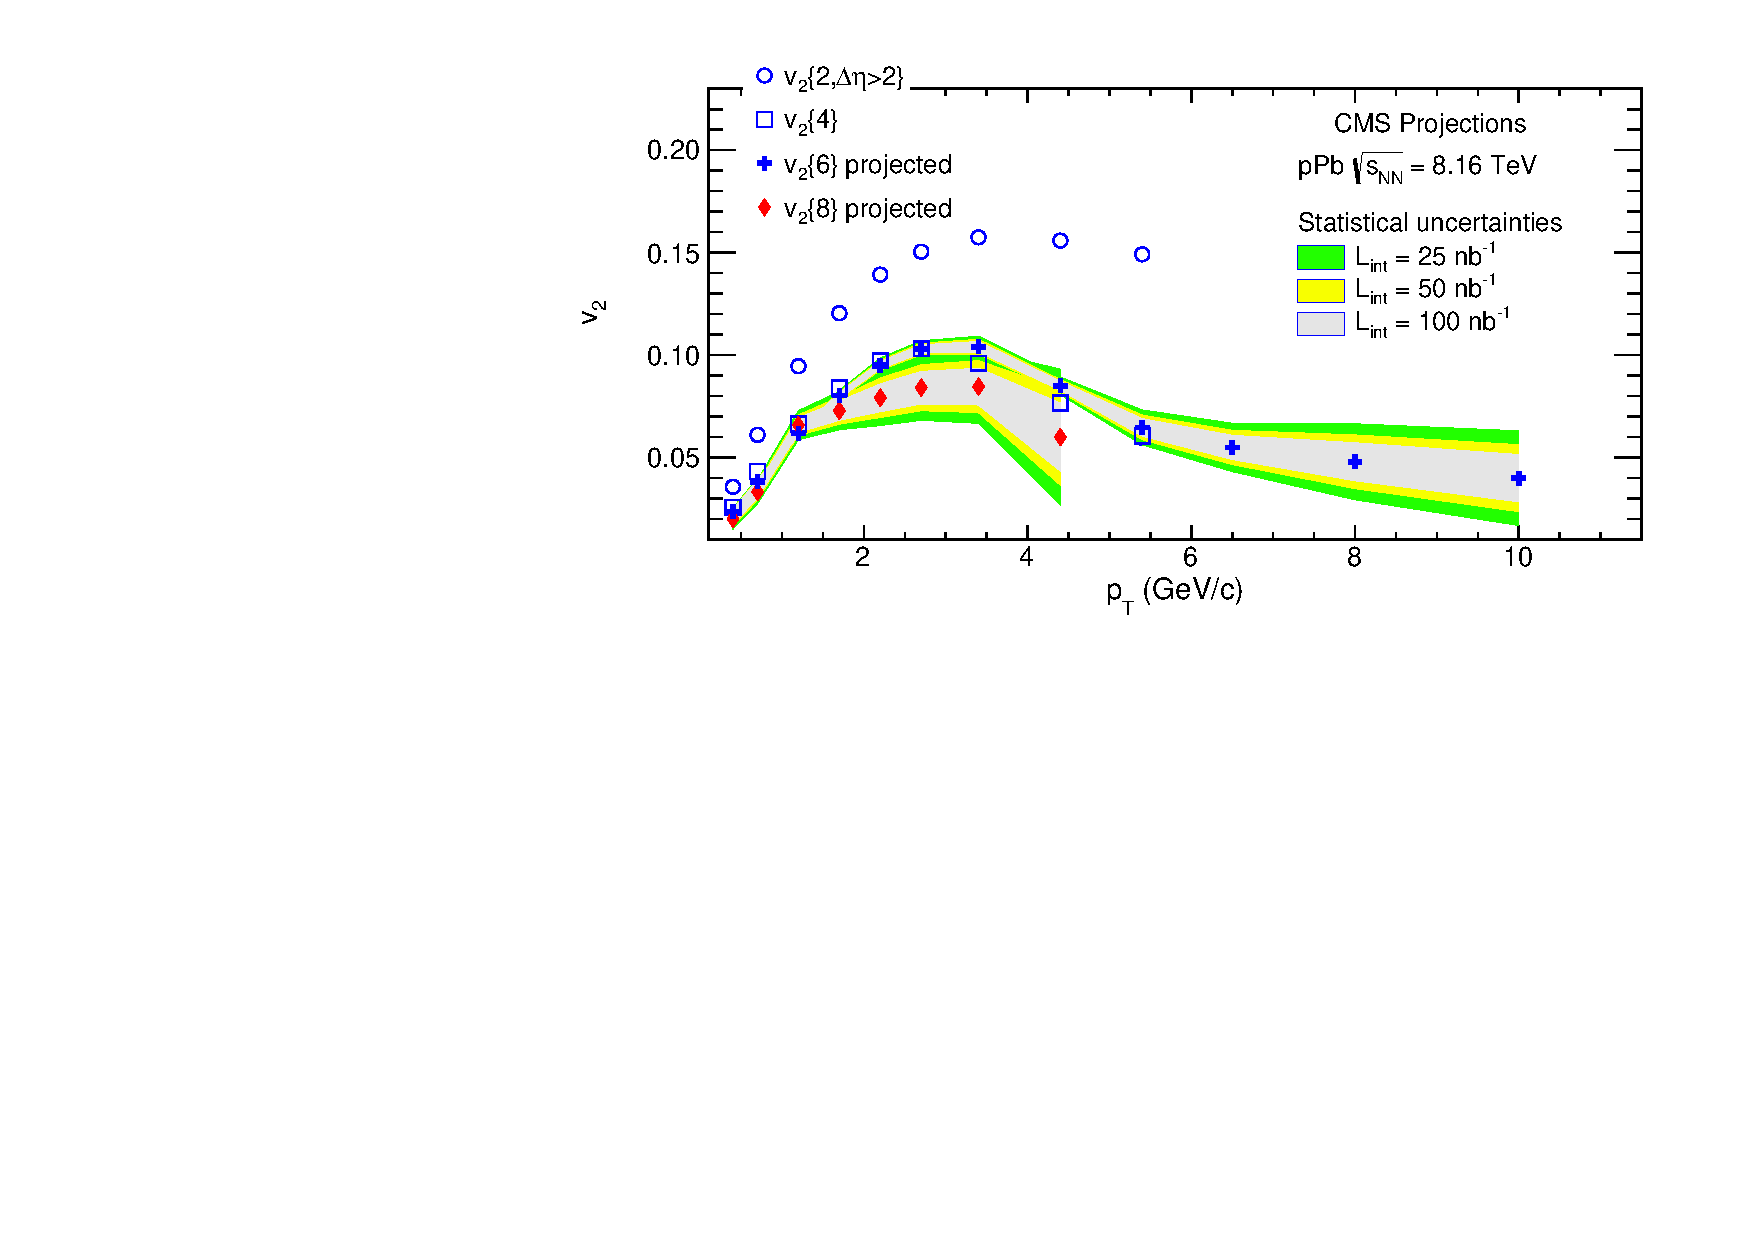
\includegraphics[width=\textwidth]{figures/vnpT_proj_100nb_combineLumi.pdf}
    \caption{ Projected statistical uncertainties of $v_2\{6\}$ and $v_2\{8\}$ as a function of \pt\ 
    for pPb collisions at \rootsNN\ = 8.16 TeV, based on data at \rootsNN\ = 5.02 TeV, with luminosity
    scenarios of L$_{\rm int}$ = 100, 50 and 25 nb$^{-1}$.
    }
    \label{fig:vnpT}
  \end{center}
\end{figure}

\begin{figure}[thb]
  \begin{center}
    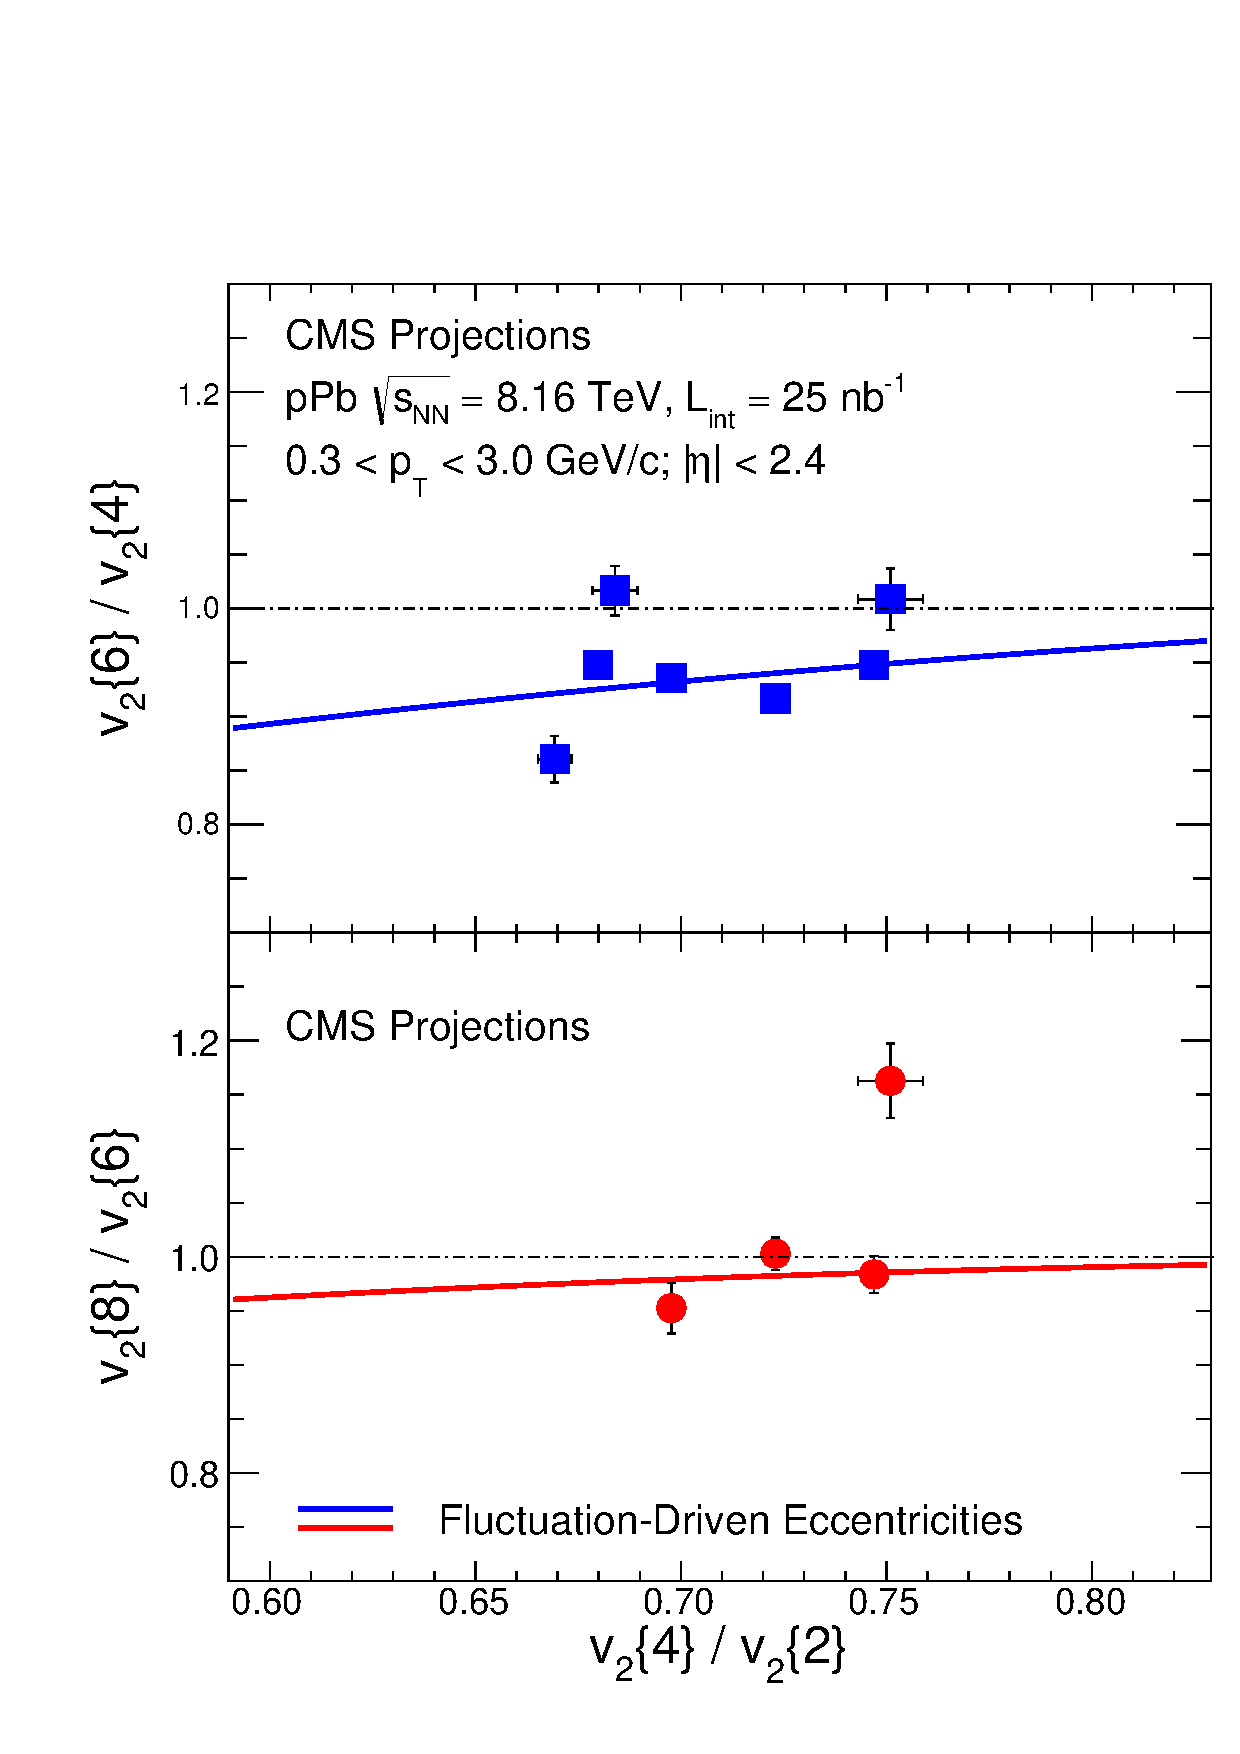
\includegraphics[width=0.5\textwidth]{figures/vnRatios_proj_100nb.pdf}
    \caption{ Projected statistical uncertainties of $v_2\{4\}/v_2\{2\}$, $v_2\{6\}/v_2\{4\}$ and $v_2\{8\}/v_2\{6\}$ ratios
    for pPb collisions at \rootsNN\ = 8.16 TeV with L$_{\rm int}$ = 100 nb$^{-1}$, based on data at \rootsNN\ = 5.02 TeV.
    }
    \label{fig:vnNtrk}
  \end{center}
\end{figure}

\clearpage